\documentclass[english,12pt,a4paper]{book}
%TODO: Correct format, not a4
\usepackage[T1]{fontenc} % In case we want special characters
\usepackage[utf8]{inputenc} % We are all writing in UTF-8

\usepackage[numbers]{natbib} % We need to tweak our referencing a bit.
\usepackage{appendix} % Fixes formatting of appendices
\usepackage[printonlyused]{acronym} % Package to handle the acronym list
\usepackage{graphicx} % We *may* use images
\graphicspath{{images/}} % and it is clean to put them in a separate dir
\usepackage{hyperref} % Internal and external links is nice
\hypersetup{pdfborder=0 0 0} % ..especially without red borders
\usepackage{amstext} % To support \text in math mode

% Packages and settings for code listings
\usepackage{listings}
\usepackage{caption}
\usepackage{upquote}
\usepackage{xcolor}
\DeclareCaptionFont{white}{\color{white}}
\DeclareCaptionFormat{listing}{\colorbox{gray}{\parbox{\textwidth}{#1#2#3}}}
\captionsetup[lstlisting]{format=listing,labelfont=white,textfont=white}
\lstset{
language=Java,
keywordstyle=\bfseries\ttfamily\color[rgb]{0,0,1},
identifierstyle=\ttfamily,
commentstyle=\color[rgb]{0.133,0.545,0.133},
stringstyle=\ttfamily\color[rgb]{0.627,0.126,0.941},
showstringspaces=false,
basicstyle=\small,
numberstyle=\footnotesize,
numbers=left,
stepnumber=1,
numbersep=10pt,
tabsize=2,
breaklines=true,
prebreak = \raisebox{0ex}[0ex][0ex]{\ensuremath{\hookleftarrow}},
breakatwhitespace=false,
aboveskip={1.5\baselineskip},
columns=fixed,
upquote=true,
extendedchars=true,
frame=bottomline,
inputencoding=utf8
}

% Set equal margins on book style
% \usepackage{layout} % Use \layout to print out the margins (debug)
\usepackage{geometry}
\geometry{bindingoffset=1cm}

% Restyle chapter headers
\usepackage{fix-cm}
\makeatletter
\renewcommand{\@makechapterhead}[1]{%
  \vspace*{50\p@}%
  {\parindent \z@ \raggedright \normalfont
    \vspace{15pt}%
    \ifnum \c@secnumdepth >\m@ne
        %\hfill\huge\scshape \@chapapp\space
        \hfill\fontsize{60}{90}\selectfont \thechapter % Chapter number
        \par\nobreak
        \vskip 20\p@
    \fi
    \interlinepenalty\@M
    \hfill \Huge \scshape #1\par % Chapter title
    \vspace{5pt}
    \hrule
    \nobreak
    \vskip 40\p@
  }}
\makeatother

\author{Eirik Haver \and Eivind Melvold \and Pål Ruud}
\title{Master thesis - Cloud Storage Vault}
\date{\today}

\begin{document}

\include{title}
\pagestyle{empty}

\chapter*{Abstract}
\addcontentsline{toc}{chapter}{Abstract}
\pagestyle{plain}
\pagenumbering{Roman}
\setcounter{page}{1}

%  Writers should follow a checklist consisting of:
% Motivation: Why do we care about the problem and results?
% Problem Statement: What problem are we trying to solve? Scope/limits.
% Approach: How did we go about solving or making progress on the problem?
% Results: What is the answer? Numbers, not vague 'very', 'small' etc.
% Conclusions: What are the implications of your answer? Further work.
%
%  Each section is typically a single sentence, although there is room for
%  creativity.

\chapter*{Preface}
\addcontentsline{toc}{chapter}{Preface}

The work behind this project report was carried out during the spring semester
in 2011 at the Norwegian University of Science and Technology (NTNU), Department
of Telematics (ITEM).
\vspace{13pt}

\begin{center}
Eirik Haver, Eivind Melvold and Pål Ruud
\vspace{13pt}

\end{center}

\tableofcontents

\cleardoublepage
\phantomsection
\addcontentsline{toc}{chapter}{\listfigurename}
\listoffigures

\cleardoublepage
\phantomsection
\addcontentsline{toc}{chapter}{\listtablename}
\listoftables

\cleardoublepage
\phantomsection
\addcontentsline{toc}{chapter}{\lstlistlistingname}
\lstlistoflistings
\cleardoublepage

\chapter*{Acronyms}
\addcontentsline{toc}{chapter}{Acronyms}

\begin{acronym}
\acro{AES}{Advanced Encryption Standard}
\acro{CA}{Certification authority}
\acro{DSA}{Digital Signature Algorithm}
\acro{DSS}{Digital Signature Scheme}
\acro{FAQ}{Frequently Asked Questions}
\acro{LAFS}{Least Authorithy File System}
\acro{PBKDF2}{Password-Based Key Derivation Function version 2}
\acro{PKI}{Public Key Infrastructure}
\acro{PGP}{Pretty Good Privacy}
\acro{RSA}{Rivest, Shamir and Adleman}
\acro{SHA}{Secure Hash Algorithm}
\acro{SSL}{Secure Socket Layer}
\acro{TLS}{Transport Layer Security}
\end{acronym}

%**************************************%
\chapter{Introduction}
%**************************************%
\pagenumbering{arabic}
\setcounter{page}{1}

\section{Method}

\section{Outline}

The work is presented as per the following chapters:

\paragraph{Chapter 2} provides background knowledge of the technologies and
software used.


%**************************************%
\chapter{Background}
%**************************************%
%-sym vs asym crypto
%    -AES, modes
%    -RSA
%-Tahoe

%- MITM
%- Brute Force
\section{Security Services}
This section briefly explains certain security services used in this
thesis. A security service is any processing or communication service that
enhances the security of the data processing systems and the information
transfers of any organization\cite[p. 12]{stallings}.

\subsection{Confidentiality} Confidentiality is the art of keeping a message
secret from unauthorized parties\cite[p. 18]{stallings}. This can typically be
done by either preventing other parties access to the message at all, or making
the contents unreadable for instance by the use of encryption. 

\subsection{Integrity}
Integrity in a security perspective deals with detecting, preventing or
recovering a message from being changes by an unauthorized party \cite[p.
18]{stallings}.

\subsection{Authentication}
Authentication is the act for a user, service or similar to prove that he is
what he claims to be\cite[p. 18]{stallings}. 

\subsection{Nonrepudiation}
Nonrepudiation prevents either sender or receiver of a message from denying a
transmitted message, in other words one party can prove the other parties
involvement\cite[p. 19]{stallings}.

\section{Cryptographic Primitives}
This section explains the low level security primitives used in this thesis.

\subsection{Encryption}
Encryption is the process of transforming some information into an unreadable
form. Encryption is primarily used to enforce Confidentially, but can also be
used for other purposes such as authentication. In a very basic form an
encryption scheme consist of an algorithm, the cipher, a key and a message, the
plaintext, that is all used to create an encrypted message, a ciphertext. If
a good cipher is used, knowledge of the cipher, plaintext and ciphertext should
not be enough to obtain the key.

\paragraph{Block-cipher and Stream-cipher} are classifications on how a cipher
treats data\cite[p. 32]{stallings}. With a block-cipher data will be encrypted
in blocks of specific sizes. If the data length is not a multiple of the block
size, the data will be padded. A stream cipher on the other hand will encrypt
the message co.

\paragraph{Symmetric encryption} is an encryption scheme where the same key is
used for both encryption and decryption\cite[p. 32]{stallings}. \ac{AES} is a
block cipher and is the current standard for symmetric encryption. \ac{AES}
works on a block of 128-bit and support keys of 128, 192 and 256-bit. 


\paragraph{Asymmetric encryption} is an encryption scheme where a different key
is used for encryption than decryption\cite[p. 259]{stallings}. An asymmetric
encryption scheme is often called a public-key encryption scheme, where one key
is defined as private and the other as public. The public key is shared to
allow other parties to encrypt messages for the owner of the private key. The
downside of asymmetric encryption compared to symmetric is that it requires a
larger key and has a larger computational overhead to obtain the same level of
confidentiality. The probably best known asymmetric cipher is \ac{RSA}.

\subsection{Cryptographic hash functions}
A cryptographic hash function is a deterministic mathematical procedure which
takes an arbitrary block of data and outputs a fixed-size bit string. The output
is referred to as the hash value, message digest or simply digest.
Another property of a cryptographic hash function is that the smallest change in
the input data (e.g. one bit) should completely change the output of the hash
function. In other words it should be infeasible to find the reverse of a
cryptographic hash function \cite[p. 335]{stallings}. It should also be infeasible to
find two blocks of data which produce the same hash value (a \emph{collision}).

The standard for cryptographic hash functions today are \ac{SHA}-1 and the
\ac{SHA}-2 family.

\section{Applications of cryptographic primitives}

\subsection{Digital Signatures}
A digital signature is the digital equivalent of a normal signature, it
verifies that an entity approves with or has written a message, the date the
signature was made and it should be verifiable by a third party \cite[p.
379]{schneier}. It should logically not be possible or at least unfeasible to
fake a digital signature. It is possible to create digital signatures with
\ac{RSA} there is also a standard for digital signatures called \ac{DSS} which
uses \ac{DSA} as the actual algorithm.

\subsection{Digital Certificates and PKI}
A digital certificate is the pairing of a digital signature and a public key.
By this scheme the services confidentiality, authentication and nonrepudiation
can be achieved.  Basically a person or other entity has a certificate with
some clues about the identity in it, e.g. the e-mail, together with a public
key. This certificate can then be signed using digital signatures to verify
that some other entity trusts this certificate. In practise the entity which
signs certificates is the \ac{CA} which all clients have the public key
information for, and trusts. The \ac{CA} will also contain information about
which certificates has been revoked, i.e. should not be trusted in use. Such a
scheme is usually referred
to as a \ac{PKI}.

\subsubsection{PGP}
\ac{PGP} is a scheme similar to \ac{PKI} but with no \ac{CA} that all users
trusts. Instead trust is made between users by somehow verifying their public
key, for instance by meeting face to face. A user can then sign another users
key, set a trust level for the user and publish this information to a
keyserver. Another user can then calculate a trust to an unknown person based
on the trust set by peoples that he trusts. 

\subsection{SSL/TLS}
\ac{TLS} and its predecessor \ac{SSL} are techniques for obtaining
confidentiality, integrity for transfer of files over a
network\cite{stallings}. It does so by a combination of different algorithms
and primitives, but a digital certificate is required for authentication. 

\subsection{PBKDF2}
%TODO: See if we actually use this.
\ac{PBKDF2} is a key derivation function to create an encryption key based on
a password. The point of this is that a password is often something that should
be memorable to a person, but what is memorable to a person might be a to short
phrase to withstand a brute force attack. What \ac{PBKDF2} does is make the
process of deriving the key from the password an expensive process in terms of
computational power, to make it more resistant to brute force attacks.

\section{Existing Solutions}
There are a number of existing storage solutions for storing data in the cloud,
with more or less of the functionality required to fulfill the problem
description for this thesis. The section highlights some of them.

\subsection{Dropbox}
Dropbox\footnote{\url{http://www.dropbox.com}} is a commercial application for
storing data in the cloud, more specific using Amazons S3 storage service. It
claims that files are stored encrypted with \ac{AES}-256 which can only be
decrypted with the users username and password, and that Dropbox employees are
not able to access the files of the user. However Dropbox also has a Forgot
password feature which means that Dropbox can read the users files if they
really want to. Their \ac{FAQ} does however say that some people have been
successfull in putting truecrypt containers in Dropbox to prevent this.

\subsection{Tahoe-LAFS}
Tahoe-\ac{LAFS}\footnote{http://www.tahoe-lafs.org} is an open source
cloud storage file system which does fulfill the requirements set by our
problem description in regards to security. In Tahoe-\ac{LAFS} files are
exclusivly encrypted client-side, before beeing uploaded into the cloud.
Tahoe-\ac{LAFS} also uses erasure-coding to obtain redundancy across multiple
storage servers.  

%**************************************%
\chapter{Architectural Solution}
%**************************************%

The architectural solution of a secure cloud file sharing system has to convince
its users that the functions indeed are secure, and that the concepts are easy
to understand and accept.

\section{Introduction}
% Concepts introduced by the system

% Picture: "Architecture: Overview"

\section{File Storage}

- Structure
- Various File access modes

\section{User scenarios}

\subsection{Upload Files}

\begin{figure}[h!]
    \centering
    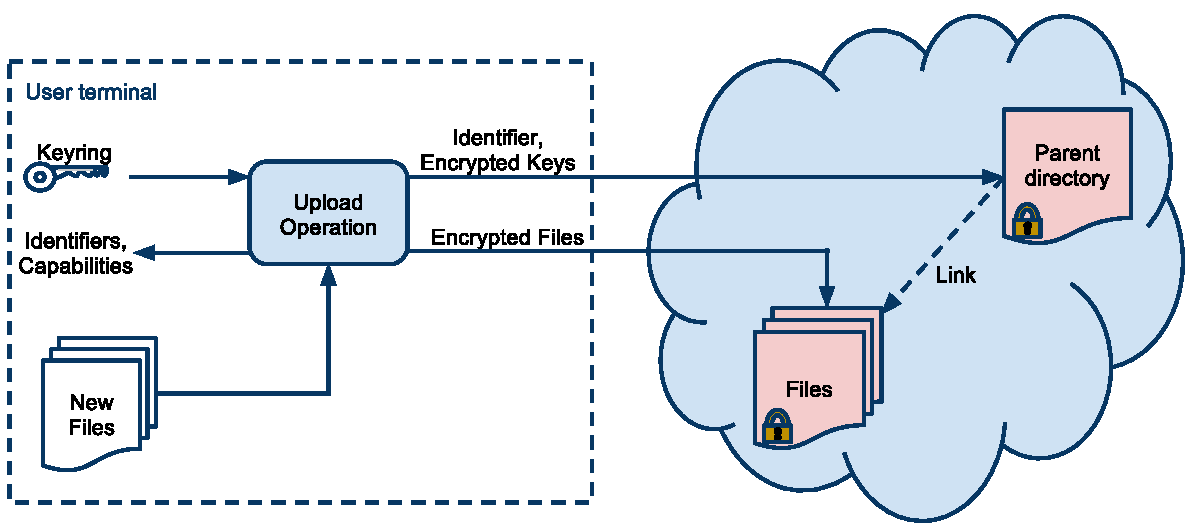
\includegraphics[width=\columnwidth]{ArchitectureUpload.pdf}
    \caption{Scenario: Uploading of files}
    \label{fig:arch:upload}
\end{figure}

\subsection{Download file}

\subsection{Share files}


%**************************************%
\chapter{Cryptographical Solutions}
%**************************************%
This chapter will elaborate on the cryptographical solutions applied to the
architectural scheme in chapter \ref{chap:AS}. We will take a closer look at
how confidentiality, integrity, authentication and access control can be 
integrated into the proposed architecture.\\

A fundamental scheme for key distribution is needed to realize the desired
security features, hence an appropriate solution for key distribution will
also be given.

-Intro - What and why?

{
-Confidentiality: AES-CBC, RSA

-Integrity: SHA-256

-Authentication: RSA PrK signature

-Key hierarchy

-Key distribution
}

%**************************************%
\chapter{Implementation}
%**************************************%

%**************************************%
\chapter{Results}
%**************************************%

%**************************************%
\chapter{Discussion}
%**************************************%

%**************************************%
\chapter{Conclusion and Future Work}
%**************************************%

% BibTeX bibliography lives in external file
\bibliographystyle{plainnat}
\bibliography{references}
% TODO: Can we fix references in order of apperance?

\appendix
\appendixpage
\addappheadtotoc
% Appendix goes here


\end{document}
